\documentclass[11pt]{article}
\usepackage[margin=0.74in]{geometry}
\geometry{letterpaper}
\usepackage{graphicx}
\usepackage{amssymb}
\usepackage{dejavu}
\usepackage{listings}
\usepackage{fancyhdr}
\pagestyle{fancy}

\graphicspath{{./images/}}

\chead{\scshape\bfseries Minesweeper Final Design}
\rhead{Tristan Seifert, Blake Powell\\ CSCE 121-502}

\lstset{
	numbers=left,
	tabsize=4,
	numberfirstline=true,
	basicstyle=\footnotesize\ttfamily,
	breaklines=true
}

\begin{document}
\section{Overall Design}
The program will be divided into four parts:

\begin{itemize}
	\item \textbf{Main Window}: This is an FLTK window that contains all the widgets for the game, and handles all user input/game status.
	\item \textbf{Game Board}: A custom FLTK widget that draws a grid of cells, and contains the data for the bombs, flags, etc.
	\item \textbf{Persistence}: Stores the high scores in a file in the program directory, and loads them when the game is started again.
	\item \textbf{New Game Dialog}: Allows the user to select which difficulty level they want to play the game at, or use a custom grid size and mine count.
\end{itemize}

Every algorithm initially outlined in the initial document was used in the \texttt{C++} code with very minor modifications, so they are reproduced below.

\section{Distribute Mines}
This algorithm will place $n$ mines randomly throughout the grid.

\begin{lstlisting}[frame=single,language=C++]
void generateMines(int n) {
	if(n > (this->gridW * this->gridH)) {
		throw runtime_error("cannot fill more mines than there are cells");
	}

	int minesPlaced = 0;

	while(minesPlaced < n) {
		// generate random X/Y coordinate
		int x = arc4random_uniform(this->gridW);
		int y = arc4random_uniform(this->gridH);

		// is there already a mine here?
		if(this->storage[x][y].isMine != true) {
			this->storage[x][y].isMine = true;
			minesPlaced++;
		}
	}
}
\end{lstlisting}

\section{Recursive Uncovering}
When a cell is uncovered with no surrounding mines, all cells adjacent to it (in an 3x3 square, with the clicked cell in the middle) are also uncovered, and so forth, until either all cells are uncovered, or a cell with an adjacent bomb is uncovered.


\begin{lstlisting}[frame=single,language=C++]
void uncoverCell(int x, int y, bool isRecursive = false) {
	Cell &t = this->storage[x][y];

	// check if this tile is flagged
	if(t.flagged == true) {
		return;
	}

	// check if this tile has been uncovered before
	if(this->uncoveredCells.contains(Point(x, y))) {
		return;
	}

	this->uncoveredCells.push_back(Point(x, y));

	// set uncovered flag
	t.uncovered = true;

	// is this a mine?
	if(t.isMine == true && !isRecursive) {
		// lmao game over
		this->_parent->gameOver();
		this->revealMines = true;

		t.bgRed = true;
	} else {
		// calculate how many mines there are around this point
		t.surroundingMines = this->minesAroundCell(x, y);

		// if clue value is zero, uncover all adjacent tiles
		if(t.surroundingMines == 0) {
			if((x - 1) >= 0 && (y - 1) >= 0) {
				this->uncoverCell((x - 1), (y - 1), true);
			}
			// top middle
			if(/*(x - 0) >= 0 &&*/ (y - 1) >= 0) {
				this->uncoverCell((x - 0), (y - 1), true);
			}
			// top right
			if((x + 1) < this->gridW && (y - 1) >= 0) {
				this->uncoverCell((x + 1), (y - 1), true);
			}

			// middle left
			if((x - 1) >= 0/* && (y - 1) >= 0*/) {
				this->uncoverCell((x - 1), (y - 0), true);
			}
			// middle right
			if((x + 1) < this->gridW/* && (y - 1) >= 0*/) {
				this->uncoverCell((x + 1), (y - 0), true);
			}

			// bottom left
			if((x - 1) >= 0 && (y + 1) < this->gridH) {
				this->uncoverCell((x - 1), (y + 1), true);
			}
			// bottom middle
			if(/*(x - 0) >= 0 &&*/ (y + 1) < this->gridH) {
				this->uncoverCell((x - 0), (y + 1), true);
			}
			// bottom right
			if((x + 1) < this->gridW && (y + 1) < this->gridH) {
				this->uncoverCell((x + 1), (y + 1), true);
			}
		}
	}
}
\end{lstlisting}


\section{Find Remaining Mines}
Determine the number of mines in the current grid. This is done by counting up all mines, then subtracting the number of flags from that count.

\begin{lstlisting}[frame=single,language=C++]
int getMinesRemaining() {
	int remaining = 0;

	// calculate the number of mines
	for(int i = 0; i < this->gridW; i++) {
		for(int j = 0; j < this->gridH; j++) {
			TileType t = this->storage[i][j];

			if(t.isMine == true) {
				remaining++;
			}
		}
	}

	// subtract the number of uncovered/flagged mines
	for(int i = 0; i < this->gridW; i++) {
		for(int j = 0; j < this->gridH; j++) {
			TileType t = this->storage[i][j];

			if(t.flagged == true || (t.isMine == true && t.uncovered == true)) {
				remaining--;
			}
		}
	}

	return remaining;
}
\end{lstlisting}

\section{Calculate Surrounding Mines}
Given a cell's $(x, y)$ coordinate, determine how many mines are surrounding it. (This is used to calculate the 'hint' value that's shown on the cells when they're uncovered.)

\begin{lstlisting}[frame=single,language=C++]
int minesAroundCell(int x, int y) {
	int mines = 0;
	if((x - 1) >= 0 && (y - 1) >= 0) {
		mines += (this->storage[(x - 1)][(y - 1)].isMine == true) ? 1 : 0;
	} if((y - 1) >= 0) {
		mines += (this->storage[(x - 0)][(y - 1)].isMine == true) ? 1 : 0;
	} if((x + 1) < this->gridW && (y - 1) >= 0) {
		mines += (this->storage[(x + 1)][(y - 1)].isMine == true) ? 1 : 0;
	} if((x - 1) >= 0) {
		mines += (this->storage[(x - 1)][(y - 0)].isMine == true) ? 1 : 0;
	} if((x + 1) < this->gridW) {
		mines += (this->storage[(x + 1)][(y - 0)].isMine == true) ? 1 : 0;
	} if((x - 1) >= 0 && (y + 1) < this->gridH) {
		mines += (this->storage[(x - 1)][(y + 1)].isMine == true) ? 1 : 0;
	} if((y + 1) < this->gridH) {
		mines += (this->storage[(x - 0)][(y + 1)].isMine == true) ? 1 : 0;
	} if((x + 1) < this->gridW && (y + 1) < this->gridH) {
		mines += (this->storage[(x + 1)][(y + 1)].isMine == true) ? 1 : 0;
	}
	return mines;
}
\end{lstlisting}

\section{Persistence}
The \texttt{ScorePersistence} class handles saving the high scores to a file, and loading them as is needed. It does this using the C++ standard \texttt{ofstream} and \texttt{ifstream} classes.

Each row in the file indicates a different difficulty level, from 0 through 2 -- beginner, intermediate, and expert. If the user choses a custom board size, they will not be allowed to save their scores.

Each line consists of a score, a tab character, and the user's name. It is read line-by-line in the code, and read using the stream input/output operators.

Below is an example score file:

\begin{lstlisting}[frame=single]
999	No Name
51	Michael Nowak is the best
999	No Name
\end{lstlisting}

Scores of $999$ indicate that no high score has been saved yet, and thus have "No Name" associated with them. (This default data is loaded if the file doesn't exist or cannot be read. When the file is next written, those default entries get written as well.)

Data is found in the \texttt{scores.dat} file.

\begin{lstlisting}[frame=single,language=C++]
// read three lines from the file
string str;
while(std::getline(in, str)) {
    int score; std::string name;

    istringstream isstr(str);
    isstr >> score >> name;

    this->data.push_back(ScoreEntry(score, name));
}
\end{lstlisting}


\begin{lstlisting}[frame=single,language=C++]
ofstream out("scores.dat");

for(int i = 0; i < 3; i++) {
    out << this->data[i].time << "\t";
    out << this->data[i].name << endl;
}
\end{lstlisting}

\pagebreak
\section{Interface}
The same graphics as in the Windows XP desktop version of Minesweeper are used. See http://courses.cse.tamu.edu/jmichael/sp16/121/project/features.php (under the Board Visualization section,) or the second design document for images.

\subsection{Main Window}
The main window is where the game is actually displayed, and is implemented in the code  by the \texttt{MainWindow} class. The user interface is contained of a menu bar, various \texttt{Fl\_Box} classes (used for the timer/mine counter) and the custom \texttt{GameBoard} class as the main view.

\begin{figure}[htbp]
   \centering
   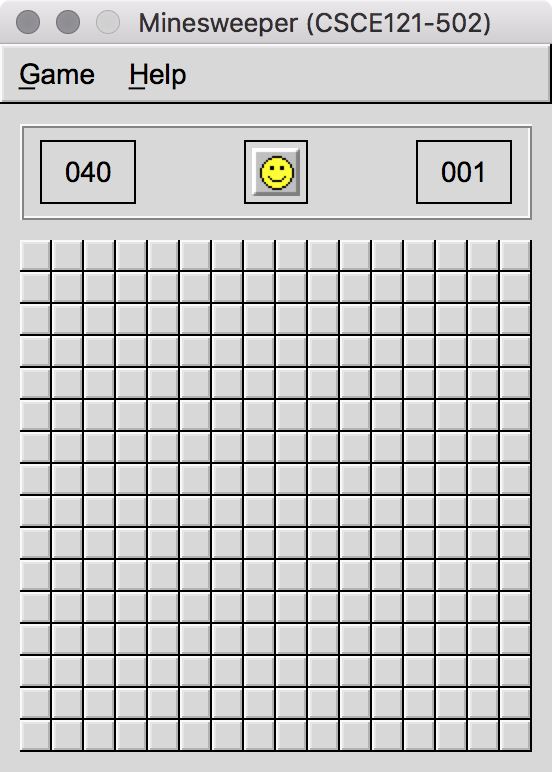
\includegraphics[width=0.32\textwidth]{main.png}
   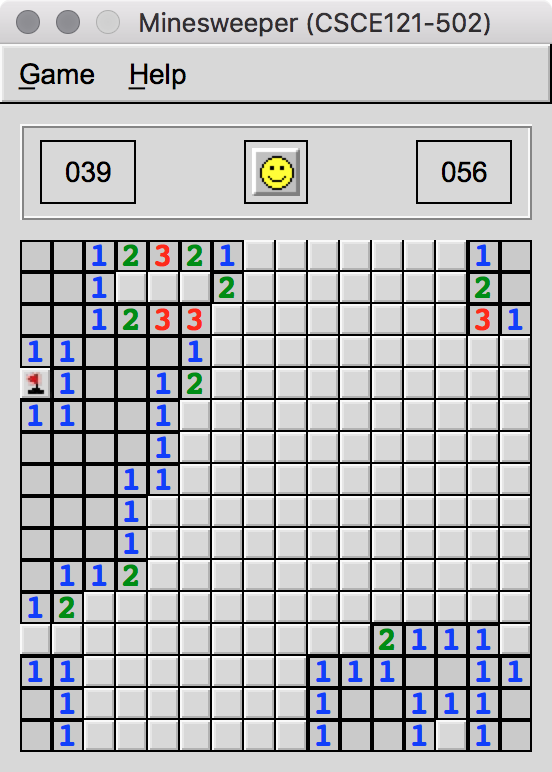
\includegraphics[width=0.32\textwidth]{mainProgress.png}
   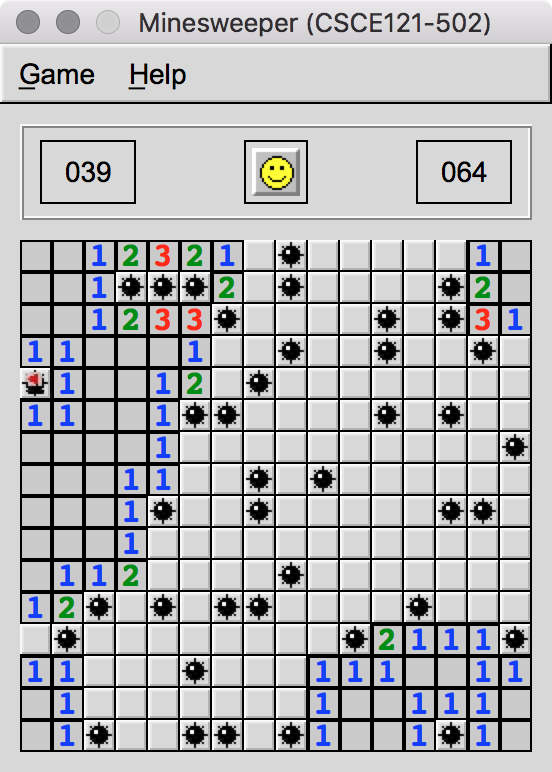
\includegraphics[width=0.32\textwidth]{mainProgressDebug.png}
   \caption{Main Window (Start of Game, During Game, Game with Debug Mode Active)}
\end{figure}

When the game is first opened (or a new game is started using the Game $\rightarrow$ New Game... menu item) a window is displayed where the user can select a difficulty level (board size and number of mines) -- Beginner (9x9, 10 mines), Intermediate (16x16, 40 mines), and Expert (16x30, 99 mines). Alternatively, the user may specify a custom board size (up to 99x99) and number of mines, up to 256.

\begin{figure}[htbp]
   \centering
   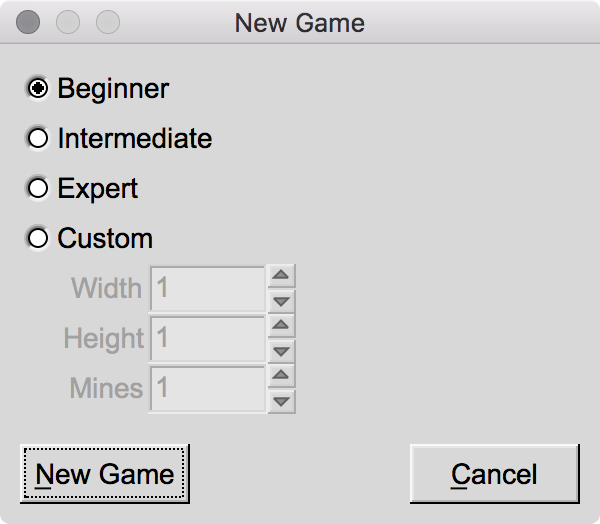
\includegraphics[width=0.35\textwidth]{newGame.png}
   \caption{Difficulty Selector}
\end{figure}

During the course of the game, fields can be left-clicked to reveal that tile. If the tile has no mines around it, all tiles adjacent to it in a 3x3 square will also be revealed, continuing until a tile has either been revealed already or is adjacent to a mine. If the tile contains a mine, the game ends.

Right-clicking a field will flag it and decrement the mine counter. Right-clicking a flag will change it to a question mark, and right-clicking a question mark will change it back into an uncovered tile that can be revealed.

\begin{figure}[htbp]
   \centering
   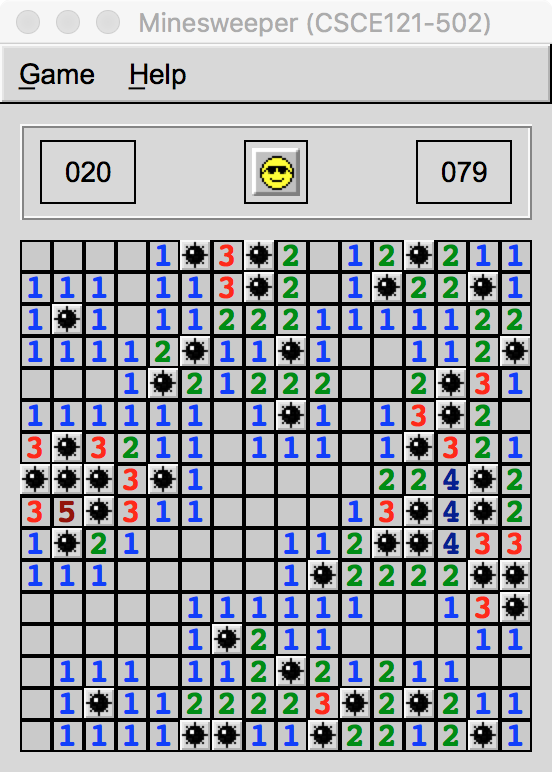
\includegraphics[width=0.32\textwidth]{mainWon.png}
   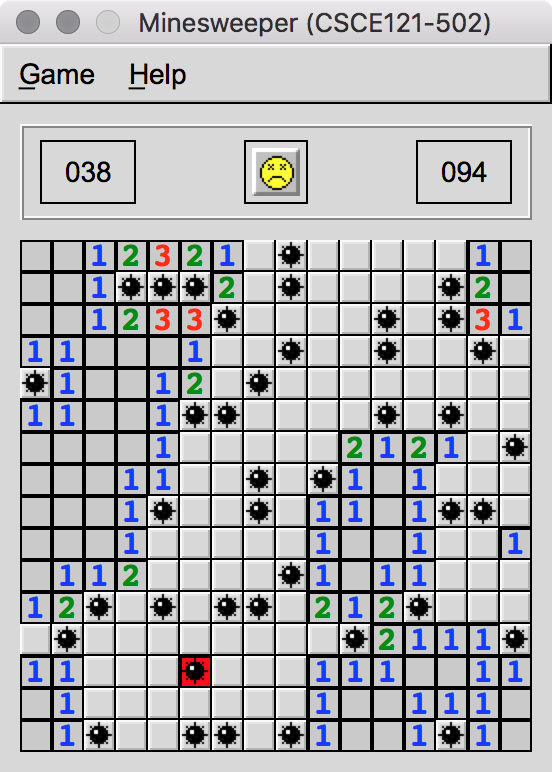
\includegraphics[width=0.32\textwidth]{mainGameOver.png}
   \caption{Main Window (Won and Game Over)}
\end{figure}

\subsection{Game Won/Game Over}
As with the original Microsoft$^{TM}$ version of Minesweeper, the smiley face at the top of the window will change to have sunglasses when the game was won. If the user's playing a preset, they will either be offered to save their name as a high score, or be notified that they didn't get a high score.

\begin{figure}[htbp]
   \centering
   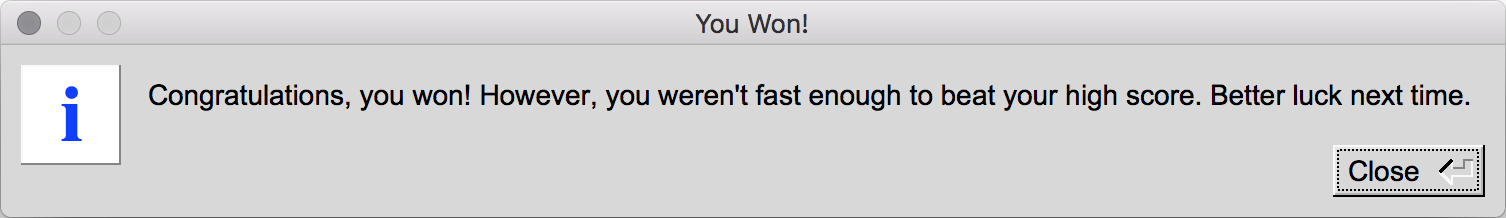
\includegraphics[width=0.95\textwidth]{wonMessage.png}
   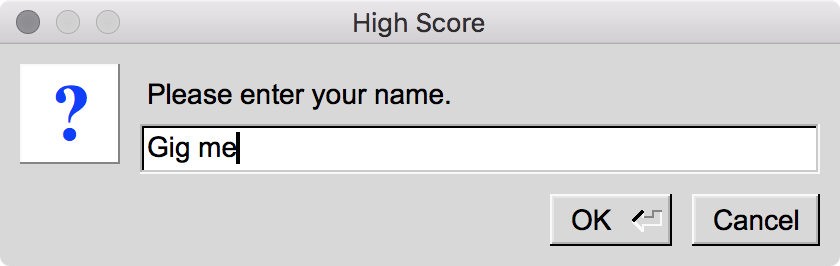
\includegraphics[width=0.6\textwidth]{newHighScore.png}
   \caption{Game Won Messages}
\end{figure}

In the case of a lost game, the face will change to a dead face, and the mine that caused the game to end is highlighted in red, and the user is notified of that fact.

\begin{figure}[htbp]
   \centering
   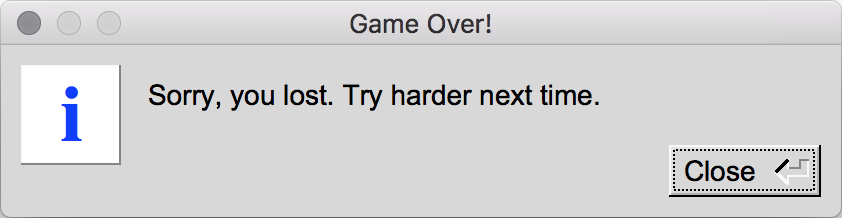
\includegraphics[width=0.65\textwidth]{gameOverMsg.png}
   \caption{Game Over Messages}
\end{figure}

\subsection{High Scores}
Whenever the user beats their best time to beat a given level, they can save their name as a high score. High scores can be viewed by using the File $\rightarrow$ High Scores... menu item. The time taken to beat the game, and their name are displayed.

\begin{figure}[htbp]
   \centering
   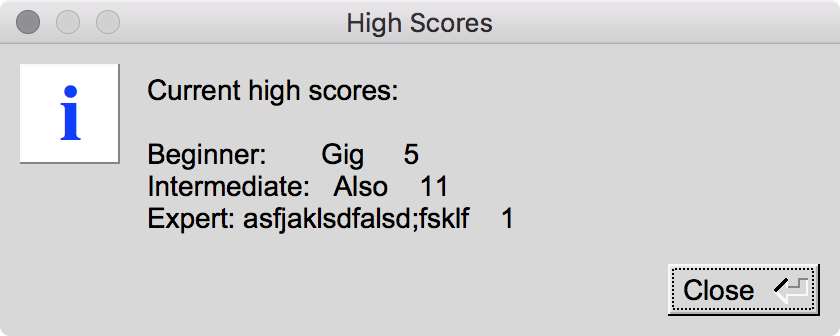
\includegraphics[width=0.6\textwidth]{highScores.png}
   \caption{High Score Viewer}
\end{figure}

\subsection{About Window}
Lastly, the program features an about window that shows the developers of the program. As with most programs, it can be accessed through the Help $\rightarrow$ About menu item.

\begin{figure}[htbp]
   \centering
   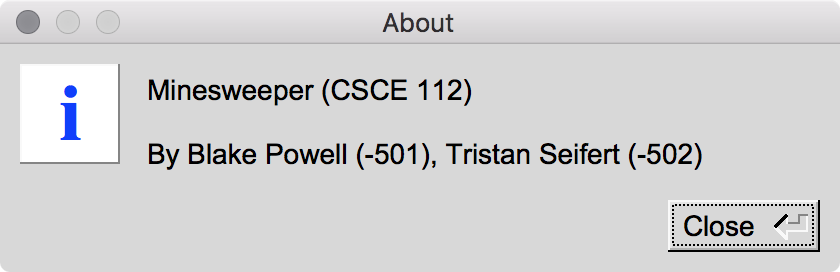
\includegraphics[width=0.6\textwidth]{about.png}
   \caption{High Score Viewer}
\end{figure}

\end{document}  